% move all configuration stuff into includes file so we can focus on the content
\documentclass[aspectratio=169,hyperref={pdfpagelabels=false,colorlinks=true,linkcolor=white,urlcolor=blue},t]{beamer}

%%%%%%%%%%%%%%%%%%%%%%%%%%%%%%%%%%%%%%%%%%%%%%%%%%%%%%%%%%%%%%%%%%%%%%%%%%%%%%%%%%
%%%%%%%%%%%%%%%%%%%%%%%%%%%%%%%%%%%%%%%%%%%%%%%%%%%%%%%%%%%%%%%%%%%%%%%%%%%%%%%%%%
% packages
\usepackage{pict2e}
\usepackage{epic}
\usepackage{amsmath,amsfonts,amssymb}
\usepackage{units}
\usepackage{fancybox}
\usepackage[absolute,overlay]{textpos} 
\usepackage{media9} % avi2flv: "C:\Program Files\ffmpeg\bin\ffmpeg.exe" -i TuneFreqFilterbank.avi -b 600k -s 441x324 -r 15 -acodec copy TuneFreqFilterbank.flv
\usepackage{animate}
\usepackage{gensymb}
\usepackage{multirow}
\usepackage{silence}
\usepackage[backend=bibtex,style=ieee]{biblatex}
\AtEveryCitekey{\iffootnote{\tiny}{}}
\addbibresource{references}

%%%%%%%%%%%%%%%%%%%%%%%%%%%%%%%%%%%%%%%%%%%%%%%%%%%%%%%%%%%%%%%%%%%%%%%%%%%%%%%%%%
%%%%%%%%%%%%%%%%%%%%%%%%%%%%%%%%%%%%%%%%%%%%%%%%%%%%%%%%%%%%%%%%%%%%%%%%%%%%%%%%%%
% relative paths
\graphicspath{{graph/}}


%%%%%%%%%%%%%%%%%%%%%%%%%%%%%%%%%%%%%%%%%%%%%%%%%%%%%%%%%%%%%%%%%%%%%%%%%%%%%%%%%%
%%%%%%%%%%%%%%%%%%%%%%%%%%%%%%%%%%%%%%%%%%%%%%%%%%%%%%%%%%%%%%%%%%%%%%%%%%%%%%%%%%
% units
\setlength{\unitlength}{1mm}

%%%%%%%%%%%%%%%%%%%%%%%%%%%%%%%%%%%%%%%%%%%%%%%%%%%%%%%%%%%%%%%%%%%%%%%%%%%%%%%%%%
%%%%%%%%%%%%%%%%%%%%%%%%%%%%%%%%%%%%%%%%%%%%%%%%%%%%%%%%%%%%%%%%%%%%%%%%%%%%%%%%%%
% theme & layout
\usetheme{Frankfurt}
\beamertemplatenavigationsymbolsempty
%\setbeamertemplate{frametitle}[smoothbars theme]
\setbeamertemplate{frametitle}
{
    \begin{beamercolorbox}[ht=1.8em,wd=\paperwidth]{frametitle}
        \vspace{-.1em}%
        \hspace{.2em}{\strut\insertframetitle\strut}
        
        \hspace{.2em}\small\strut\insertframesubtitle\strut
        %\hfill
        %
\includegraphics[height=.8cm,keepaspectratio]{CenterMusicTechnology-solid-2lines-white-CoAtag}
        
    \end{beamercolorbox}
    \begin{textblock*}{100mm}(11.6cm,.7cm)
        \includegraphics[height=.8cm,keepaspectratio]{logo_GTCMT_black}
    \end{textblock*}
}

% set this to ensure bulletpoints without subsections
\usepackage{remreset}
\makeatletter
\@removefromreset{subsection}{section}
\makeatother
\setcounter{subsection}{1}

%---------------------------------------------------------------------------------
% appearance
\setbeamercolor{structure}{fg=gtgold}
\setbeamercovered{transparent} %invisible
\setbeamercolor{bibliography entry author}{fg=black}
\setbeamercolor*{bibliography entry title}{fg=black}
\setbeamercolor*{bibliography entry note}{fg=black}

%\usepackage{pgfpages}
%\setbeameroption{show notes}
%\setbeameroption{show notes on second screen=right}
%---------------------------------------------------------------------------------
% fontsize
\let\Tiny=\tiny

%%%%%%%%%%%%%%%%%%%%%%%%%%%%%%%%%%%%%%%%%%%%%%%%%%%%%%%%%%%%%%%%%%%%%%%%%%%%%%%%%%
%%%%%%%%%%%%%%%%%%%%%%%%%%%%%%%%%%%%%%%%%%%%%%%%%%%%%%%%%%%%%%%%%%%%%%%%%%%%%%%%%%
% warnings
\pdfsuppresswarningpagegroup=1
\WarningFilter{biblatex}{Patching footnotes failed}
\WarningFilter{latexfont}{Font shape}
\WarningFilter{latexfont}{Some font shapes}
\WarningFilter{gensymb}{Not defining}


%%%%%%%%%%%%%%%%%%%%%%%%%%%%%%%%%%%%%%%%%%%%%%%%%%%%%%%%%%%%%%%%%%%%%%%%%%%%%%%%%%
%%%%%%%%%%%%%%%%%%%%%%%%%%%%%%%%%%%%%%%%%%%%%%%%%%%%%%%%%%%%%%%%%%%%%%%%%%%%%%%%%%
% title information
\title[]{Introduction to Audio Content Analysis}   
\author[alexander lerch]{alexander lerch} 
%\institute{~}
%\date[Alexander Lerch]{}
\titlegraphic{\vspace{-16mm}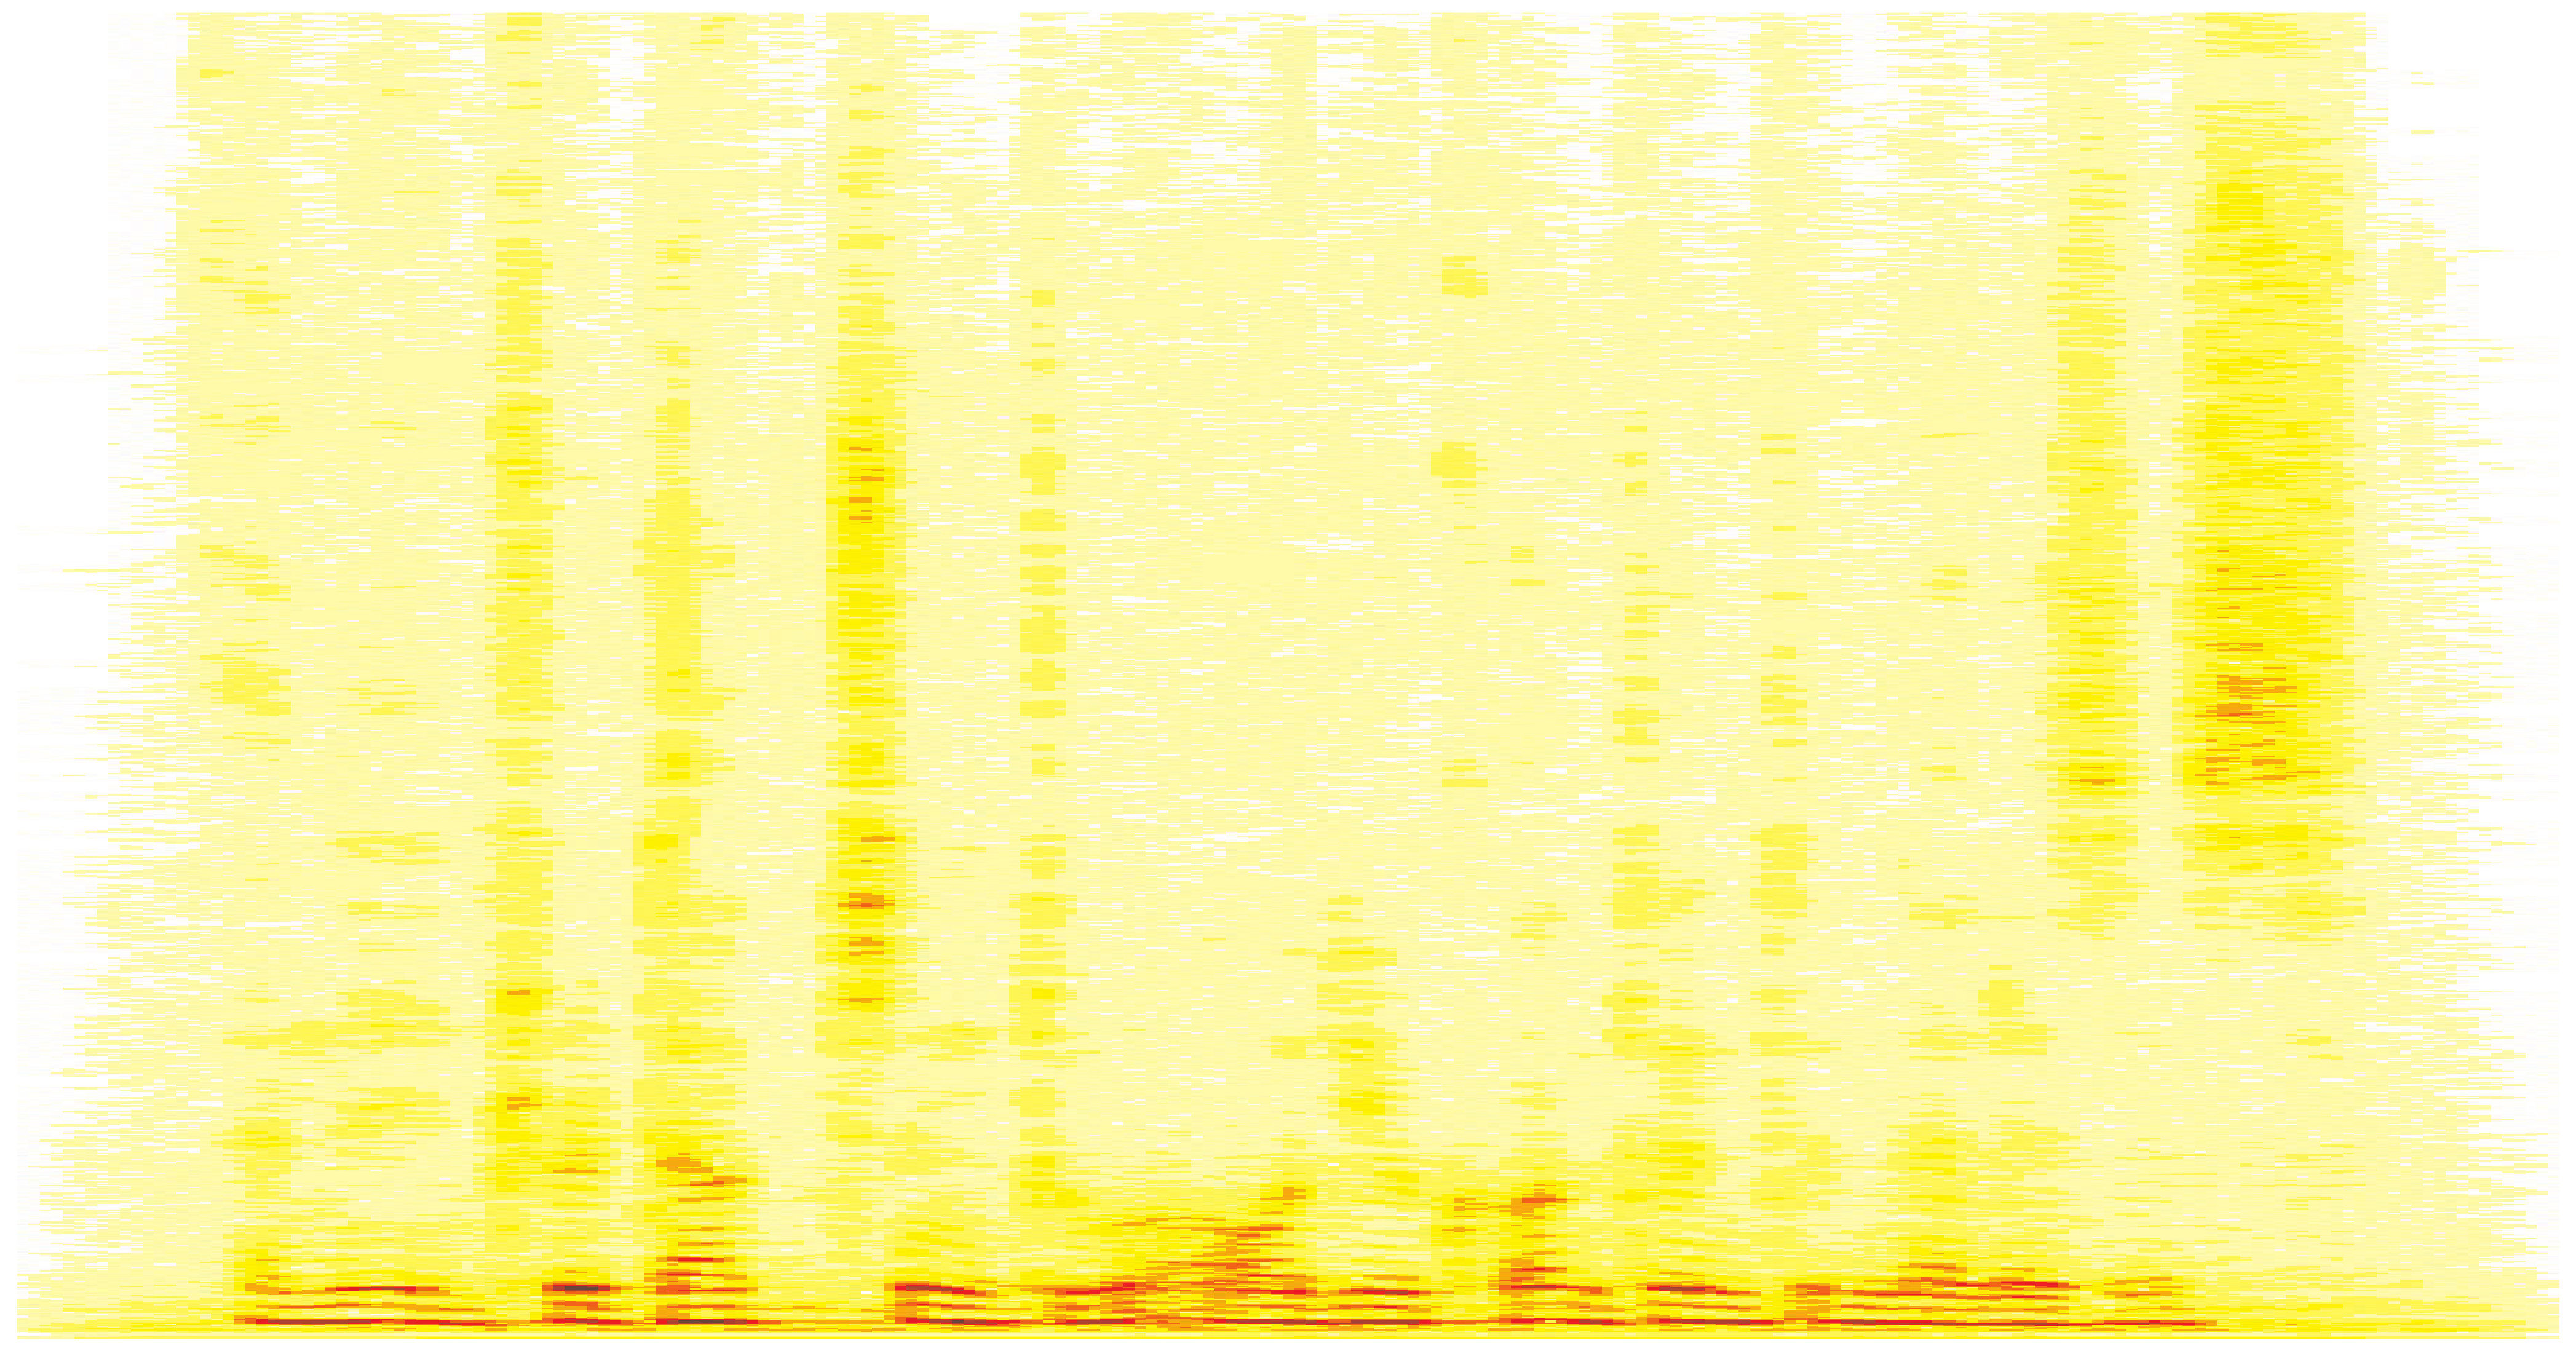
\includegraphics[width=\textwidth,height=3cm]{title}}

%%%%%%%%%%%%%%%%%%%%%%%%%%%%%%%%%%%%%%%%%%%%%%%%%%%%%%%%%%%%%%%%%%%%%%%%%%%%%%%%%%
%%%%%%%%%%%%%%%%%%%%%%%%%%%%%%%%%%%%%%%%%%%%%%%%%%%%%%%%%%%%%%%%%%%%%%%%%%%%%%%%%%
% colors
\definecolor{gtgold}{HTML}{E0AA0F} %{rgb}{0.88,0.66,1,0.06} [234, 170, 0]/256

%%%%%%%%%%%%%%%%%%%%%%%%%%%%%%%%%%%%%%%%%%%%%%%%%%%%%%%%%%%%%%%%%%%%%%%%%%%%%%%%%%
%%%%%%%%%%%%%%%%%%%%%%%%%%%%%%%%%%%%%%%%%%%%%%%%%%%%%%%%%%%%%%%%%%%%%%%%%%%%%%%%%%
% math
\DeclareMathOperator*{\argmax}{argmax}
\DeclareMathOperator*{\argmin}{argmin}
\DeclareMathOperator*{\atan}{atan}
\DeclareMathOperator*{\arcsinh}{arcsinh}
\DeclareMathOperator*{\sign}{sign}
\DeclareMathOperator*{\tcdf}{tcdf}
\DeclareMathOperator*{\si}{sinc}
\DeclareMathOperator*{\princarg}{princarg}
\DeclareMathOperator*{\arccosh}{arccosh}
\DeclareMathOperator*{\hwr}{HWR}
\DeclareMathOperator*{\flip}{flip}
\DeclareMathOperator*{\sinc}{sinc}
\DeclareMathOperator*{\floor}{floor}
\newcommand{\e}{{e}}
\newcommand{\jom}{\mathrm{j}\omega}
\newcommand{\jOm}{\mathrm{j}\Omega}
\newcommand   {\mat}[1]    		{\boldsymbol{\uppercase{#1}}}		%bold
\renewcommand {\vec}[1]    		{\boldsymbol{\lowercase{#1}}}		%bold

%%%%%%%%%%%%%%%%%%%%%%%%%%%%%%%%%%%%%%%%%%%%%%%%%%%%%%%%%%%%%%%%%%%%%%%%%%%%%%%%%%
%%%%%%%%%%%%%%%%%%%%%%%%%%%%%%%%%%%%%%%%%%%%%%%%%%%%%%%%%%%%%%%%%%%%%%%%%%%%%%%%%%
% media9
\newcommand{\includeaudio}[1]{{\includemedia[
                        addresource=audio/#1.mp3,
                        width=5mm,
                        height=5mm,
                        activate=onclick,
                        flashvars={
                            source=audio/#1.mp3  
                            &autoPlay=true
                        }]
                        {
\includegraphics[width=5mm, height=5mm]{SpeakerIcon}}
                        {APlayer.swf}}}
\newcommand{\audioautoplay}[1]{{\begin{center}\includemedia[
                            addresource=audio/#1.mp3,
                            width=.1\linewidth,
                            height=.01\linewidth,
                            activate=pageopen,
                            flashvars={
                                source=audio/#1.mp3  
                                &autoPlay=true
                            }]
                            {}
                            {APlayer.swf}\end{center}}}

\newcommand{\includevideo}[1]{{\begin{center}\includemedia[
                        addresource=video/#1.mp4,
                        width=0.8\linewidth,
                        height=0.4\linewidth,
                        activate=onclick,
                        flashvars={
                            source=video/#1.mp4  
                            &autoPlay=true
                        }]
                        {}
                        {VPlayer.swf}\end{center}}}
\newcommand{\videowithmatlab}[1]{{\begin{center}\includemedia[
                        addresource=video/animate#1.mp4,
                        width=0.8\linewidth,
                        height=0.4\linewidth,
                        activate=onclick,
                        flashvars={
                            source=video/animate#1.mp4  
                            &autoPlay=true
                        }]
                        {}
                        {VPlayer.swf}\end{center}\addreference{matlab source: matlab/animate#1.m}}}
                        

%%%%%%%%%%%%%%%%%%%%%%%%%%%%%%%%%%%%%%%%%%%%%%%%%%%%%%%%%%%%%%%%%%%%%%%%%%%%%%%%%%
%%%%%%%%%%%%%%%%%%%%%%%%%%%%%%%%%%%%%%%%%%%%%%%%%%%%%%%%%%%%%%%%%%%%%%%%%%%%%%%%%%
% other commands
\newcommand{\question}[1]{%\vspace{-4mm}
                          \setbeamercovered{invisible}
                          \begin{columns}[T]
                            \column{.8\textwidth}
                                \textbf{#1}
                            \column{.2\textwidth}
                                \vspace{-8mm}
                                \begin{flushright}
                                     
\includegraphics[scale=.5]{question_mark}
                                \end{flushright}
                                \vspace{6mm}
                          \end{columns}\pause\vspace{-12mm}}

\newcommand{\toremember}[1]{%\vspace{-4mm}
                          \begin{columns}[T]
                            \column{.8\textwidth}
                                \textbf{#1}
                            \column{.2\textwidth}
                                \vspace{-4mm}
                                \begin{flushright}
                                     
\includegraphics[scale=.5]{exclamation_mark}
                                \end{flushright}
                                \vspace{6mm}
                          \end{columns}\vspace{-6mm}}

\newcommand{\matlabexercise}[1]{%\vspace{-4mm}
                          \setbeamercovered{invisible}
                          \begin{columns}[T]
                            \column{.8\textwidth}
                                \textbf{matlab exercise}: #1
                            \column{.2\textwidth}
                                \begin{flushright}
                                     
\includegraphics[scale=.5]{logo_matlab}
                                \end{flushright}
                                %\vspace{6mm}
                          \end{columns}}

\newcommand{\addreference}[1]{  
                  
                    \begin{textblock*}{\baselineskip }(1.12\textwidth,.3\textheight) %(1.15\textwidth,.4\textheight)
                        \rotatebox{90}{\tiny {#1}}
                    \end{textblock*}}
                    
\newcommand{\figwithmatlab}[1]{
                    \begin{figure}
                        \centering
                        \includegraphics{#1}
                        %\label{fig:#1}
                    \end{figure}
                    
                    \addreference{matlab source: \href{https://github.com/alexanderlerch/ACA-Slides/blob/master/matlab/display#1.m}{matlab/display#1.m}}}
\newcommand{\figwithref}[2]{
                    \begin{figure}
                        \centering
                        \includegraphics{#1}
                        \label{fig:#1}
                    \end{figure}
                    
                    \addreference{#2}}  
                                    
\newcommand{\inserticon}[1]{

                    \begin{textblock*}{100mm}(14.5cm,7.5cm)
                        \includegraphics[height=.8cm,keepaspectratio]{#1}
                    \end{textblock*}}            

%%%%%%%%%%%%%%%%%%%%%%%%%%%%%%%%%%%%%%%%%%%%%%%%%%%%%%%%%%%%%%%%%%%%%%%%%%%%%%%%%%
%%%%%%%%%%%%%%%%%%%%%%%%%%%%%%%%%%%%%%%%%%%%%%%%%%%%%%%%%%%%%%%%%%%%%%%%%%%%%%%%%%
% counters
\newcounter{i}
\newcounter{j}
\newcounter{iXOffset}
\newcounter{iYOffset}
\newcounter{iXBlockSize}
\newcounter{iYBlockSize}
\newcounter{iYBlockSizeDiv2}
\newcounter{iDistance}



\subtitle{Module 2.2: Fundamentals~---~Quantization}

%%%%%%%%%%%%%%%%%%%%%%%%%%%%%%%%%%%%%%%%%%%%%%%%%%%%%%%%%%%%%%%%%%%%%%%%%%%%
\begin{document}
    % generate title page
	

\begin{frame}
    \titlepage
    %\vspace{-5mm}
    \begin{flushright}
        \href{http://www.gtcmt.gatech.edu}{\includegraphics[height=.8cm,keepaspectratio]{logo_GTCMT_black}}
    \end{flushright}
\end{frame}


    \section[overview]{lecture overview}
        \begin{frame}{introduction}{overview}
            \begin{block}{corresponding textbook section}
                    \href{http://ieeexplore.ieee.org/xpl/articleDetails.jsp?tp=&arnumber=6331119&}{Chapter 2~---~Fundamentals}: pp.~11--13
            \end{block}

            \begin{itemize}
                \item   \textbf{lecture content}
                    \begin{itemize}
                        \item   discretization of signals in amplitude
                        \item   properties of the quantization error
                        \item   number representation in Matlab
                    \end{itemize}
                \bigskip
                \item<2->   \textbf{learning objectives}
                    \begin{itemize}
                        \item   understanding the principle and impact of quantization
                        \item   representing audio signals in Matlab
                    \end{itemize}
            \end{itemize}
            \inserticon{directions}
        \end{frame}
        
    \section[intro]{introduction}
        \begin{frame}{digital signals}{introduction}
            \textit{digital} signals are represented with a limited number of values
            
            \bigskip
            $\Rightarrow$
            \begin{enumerate}
                \item	\textbf{sampling}: time discretization
                
                continuous time $\mapsto$ discrete equidistant points in time 
                
                
                \smallskip
                \item	{\color{gtgold}\textbf{quantization}}: amplitude discretization
                
                continuous amplitude $\mapsto$ discrete, pre-defined, set of values
            \end{enumerate}
        \end{frame}
        
        \begin{frame}{digital signals}{quantization}
            \vspace{-3mm}
            \begin{itemize}
                \item   continuous amplitude values are mapped to pre-defined, equidistant set of values
                %\item<2->   quantization steps are most frequently \textbf{equidistant}
                \item<1->   signal stored in binary $\Rightarrow$ \# quantization steps equals \textbf{power of 2}
                \smallskip
                \item<2->   \textbf{example: 4-bit quantization}
                    \begin{itemize}
                        \item	\textit{word length}: $w = \log_2(\mathcal{M}) = \unit[4]{bit}$
                        \item	\textit{number of quantization steps}: $\mathcal{M} = 2^w = 16$
                    \end{itemize}
            \end{itemize}
            
            \vspace{-3mm}
            \visible<2->{
            \figwithmatlab{Quantization}}
        \end{frame}	

        \begin{frame}{digital signals}{quantization wordlength}
            \question{What are typical wordlengths?}
            
            \begin{itemize}
                \item	\unit[8]{bit}: speech
                \item	\unit[12--14]{bit}: low quality audio/music
                \item	\unit[16]{bit}: (consumer) audio/music
                \item	\unit[$>$16]{bit}: production audio
            \end{itemize}
            \pause
            
            \bigskip
            \begin{table}
                \centering
                    \begin{tabular}{l|ccccc}
                        $w$ & \unit[16]{bit} & \unit[12]{bit} & \unit[8]{bit} & \unit[4]{bit} &\unit[2]{bit}\\
                        & \includeaudio{quantized_16}& \includeaudio{quantized_12}& \includeaudio{quantized_8}& \includeaudio{quantized_4}& \includeaudio{quantized_2} \\
                    \end{tabular}
            \end{table}
            \inserticon{audio}
        \end{frame}	

    \section[error]{quantization error}
        \begin{frame}{digital signals}{quantization error}
            \begin{figure}
                \begin{footnotesize}
				\begin{picture}(90,15)
					\setcounter{iXOffset}{0}
					\setcounter{iYOffset}{0}
					\setcounter{iXBlockSize}{10}
					\setcounter{iYBlockSize}{10}
					\setcounter{iYBlockSizeDiv2}{5}
					\setcounter{iDistance}{5}
	
					\addtocounter{iYOffset}{\value{iYBlockSizeDiv2}}
	
					\put(\value{iXOffset}, \value{iYOffset})
						{\text{$x(i)$}}
					\addtocounter{iXOffset}{1}
	
					\addtocounter{iXOffset}{\value{iDistance}}
	
					\put(\value{iXOffset}, \value{iYOffset})
						{\vector(1,0){\value{iDistance}}}
	
					\addtocounter{iXOffset}{\value{iDistance}}
					\addtocounter{iYOffset}{-\value{iYBlockSizeDiv2}}
					
					\put(\value{iXOffset}, \value{iYOffset})
						{\framebox(\value{iXBlockSize}, \value{iYBlockSize}) {Q}}
	
					\addtocounter{iXOffset}{\value{iXBlockSize}}
					\addtocounter{iYOffset}{\value{iYBlockSizeDiv2}}
	
					\put(\value{iXOffset}, \value{iYOffset})
						{\vector(1,0){\value{iDistance}}}
	
					\addtocounter{iXOffset}{\value{iDistance}}
					\addtocounter{iXOffset}{1}

					\put(\value{iXOffset}, \value{iYOffset})
						{\text{$x_\mathrm{Q}(i)$}}


					\setcounter{iYOffset}{0}
					\addtocounter{iXOffset}{20}
					\addtocounter{iYOffset}{\value{iYBlockSizeDiv2}}
	
					\put(\value{iXOffset}, \value{iYOffset})
						{\text{$x(i)$}}
					\addtocounter{iXOffset}{1}
	
					\addtocounter{iXOffset}{\value{iDistance}}
					\put(\value{iXOffset}, \value{iYOffset})
						{\vector(1,0){\value{iDistance}}}

                    \put(57.3, 4.2)
                        {$\oplus$}

					\put(58.5, 10.6)
						{\vector(0,-1){\value{iDistance}}}

					\put(59, 11)
						{\text{$q(i)$}}
					
                    \addtocounter{iXOffset}{\value{iDistance}}
                    \addtocounter{iXOffset}{1}
					\put(\value{iXOffset}, \value{iYOffset})
						{\vector(1,0){\value{iDistance}}}

					\addtocounter{iXOffset}{\value{iDistance}}
					\addtocounter{iXOffset}{1}

					\put(\value{iXOffset}, \value{iYOffset})
						{\text{$x_\mathrm{Q}(i) = x(i) + q(i)$}}
				\end{picture}
\end{footnotesize}

            \end{figure}
            \bigskip
            \pause
            
            model for quantization: \\
            quantization noise $q$ is added to input signal $x$
            \begin{eqnarray*}
                x_{\mathrm{Q}}(i)   &=& x(i) + q(i)\\
                q(i) &=& x(i) - x_{\mathrm{Q}}(i)
            \end{eqnarray*}
        \end{frame}		
        \begin{frame}{digital signals}{quantization error magnitude}
            \question{What is the maximum amplitude of the quantization error?}

            \figwithmatlab{QuantizationError}
        \end{frame}	

        \begin{frame}{digital signals}{quantization error properties}
            Under the assumption that the signal has a variance much higher than the quantization step size (no derivation), we find that the quantization error
            \begin{itemize}
                \item   is white noise and uncorrelated to signal,
                \item   is uniformly distributed, and
                \item   its power $W_\mathrm{Q}$ is directly related to the wordlength.
            \end{itemize}
            
            \pause
            \bigskip
            The quantizer quality is usually given by its \textit{Signal-to-Noise Ratio (SNR)}
			\begin{equation*}\label{eq:snr}
				SNR = 10\cdot\log_{10}\left(\frac{W_{\mathrm{S}}}{W_{\mathrm{Q}}}\right)\; [dB] 
			\end{equation*}
        \end{frame}	
        
        \begin{frame}{digital signals}{quantization: SNR}
            \vspace{-3mm}
            \toremember{}
            \begin{block}{signal-to-noise ratio (quantizer)}
                \centering
                \begin{equation*}
                    SNR = 6.02\cdot w + c_{\mathrm{S}}\quad [dB]
                \end{equation*}
                \vspace{-5mm}
                \begin{itemize}
                    \item	every additional bit adds app.\ \unit[6]{dB} SNR
                    \item	constant $c_{\mathrm{S}}$ depends on \textit{signal} (scaling and PDF)
                \end{itemize}
            \end{block}
            \pause
            \begin{itemize}
                \item	square wave (full scale): $c_{\mathrm{S}} =  \unit[10.80]{dB}$
                \item	sinusoidal wave (full scale): $c_{\mathrm{S}} =  \unit[1.76]{dB}$
                \item	rectangular {PDF} (full scale): $c_{\mathrm{S}} =  \unit[0]{dB}$
                \item	Gaussian {PDF} (full scale = $4\sigma_{g}$): $c_{\mathrm{S}} =  \unit[-7.27]{dB}$
            \end{itemize}
        \end{frame}		
           
    \section[discrete amplitude range]{amplitude range of a discrete signal}
        \begin{frame}{digital signals}{amplitude in DSP}
            \begin{itemize}
                \item<1->   when represented as integer, different wordlengths lead to different maximum amplitude ranges
                \item<2->	most common: normalize to the absolute maximum integer value and represent the signal in \textbf{floating point format}
                \item<3->[$\Rightarrow$]   signal amplitude:
                    \begin{equation*}
                        -1 \leq x_{\mathrm{Q}} < 1
                    \end{equation*}
                \item<3->[$\Rightarrow$]	level: \\
                    \begin{center}max.\ amplitude $\mapsto \unit{0}{dBFS}$\end{center}
                \item<4->   floating point representation
                    \begin{equation*}
                        x_{\mathrm{Q}} = M_{\mathrm{G}}\cdot 2^{E_{\mathrm{G}}}
                    \end{equation*}
                \item<5->   internal float point representation usually treated as signal being \textbf{not quantized}
            \end{itemize}
        \end{frame}

    \section{summary}
        \begin{frame}{summary}{lecture content}
            \begin{itemize}
                \item  \textbf{quantization process}
                    \begin{itemize}
                        \item   modeled as addition of noise
                    \end{itemize}
                \bigskip
                \item      \textbf{quantization error properties}
                    \begin{itemize}
                        \item   maximum amplitude is half the step size
                        \item   number of steps depends on wordlength
                    \end{itemize}
                \bigskip
                \item      \textbf{SNR}
                    \begin{itemize}
                        \item   SNR depends on input signal characteristic and wordlength
                        \item   SNR increases linearly (\unit[6]{dB}/bit) with wordlength
                    \end{itemize}
                \bigskip
                \item      \textbf{signals in Matlab}
                    \begin{itemize}
                        \item   maximum amplitude independent of wordlength (-1\ldots 1)
                    \end{itemize}
            \end{itemize}
            \inserticon{summary}
        \end{frame}
\end{document}
